
\section{Methodology}
In this section, we will provide a detailed explanation on not only the modeling of road correlation, i.e. the derivation of road correlation matrix $C$, but also how to integrate it into traffic state prediction. The overall structure is shown in figure \ref{fig: model}.

\begin{figure}[htb]
    \centering
    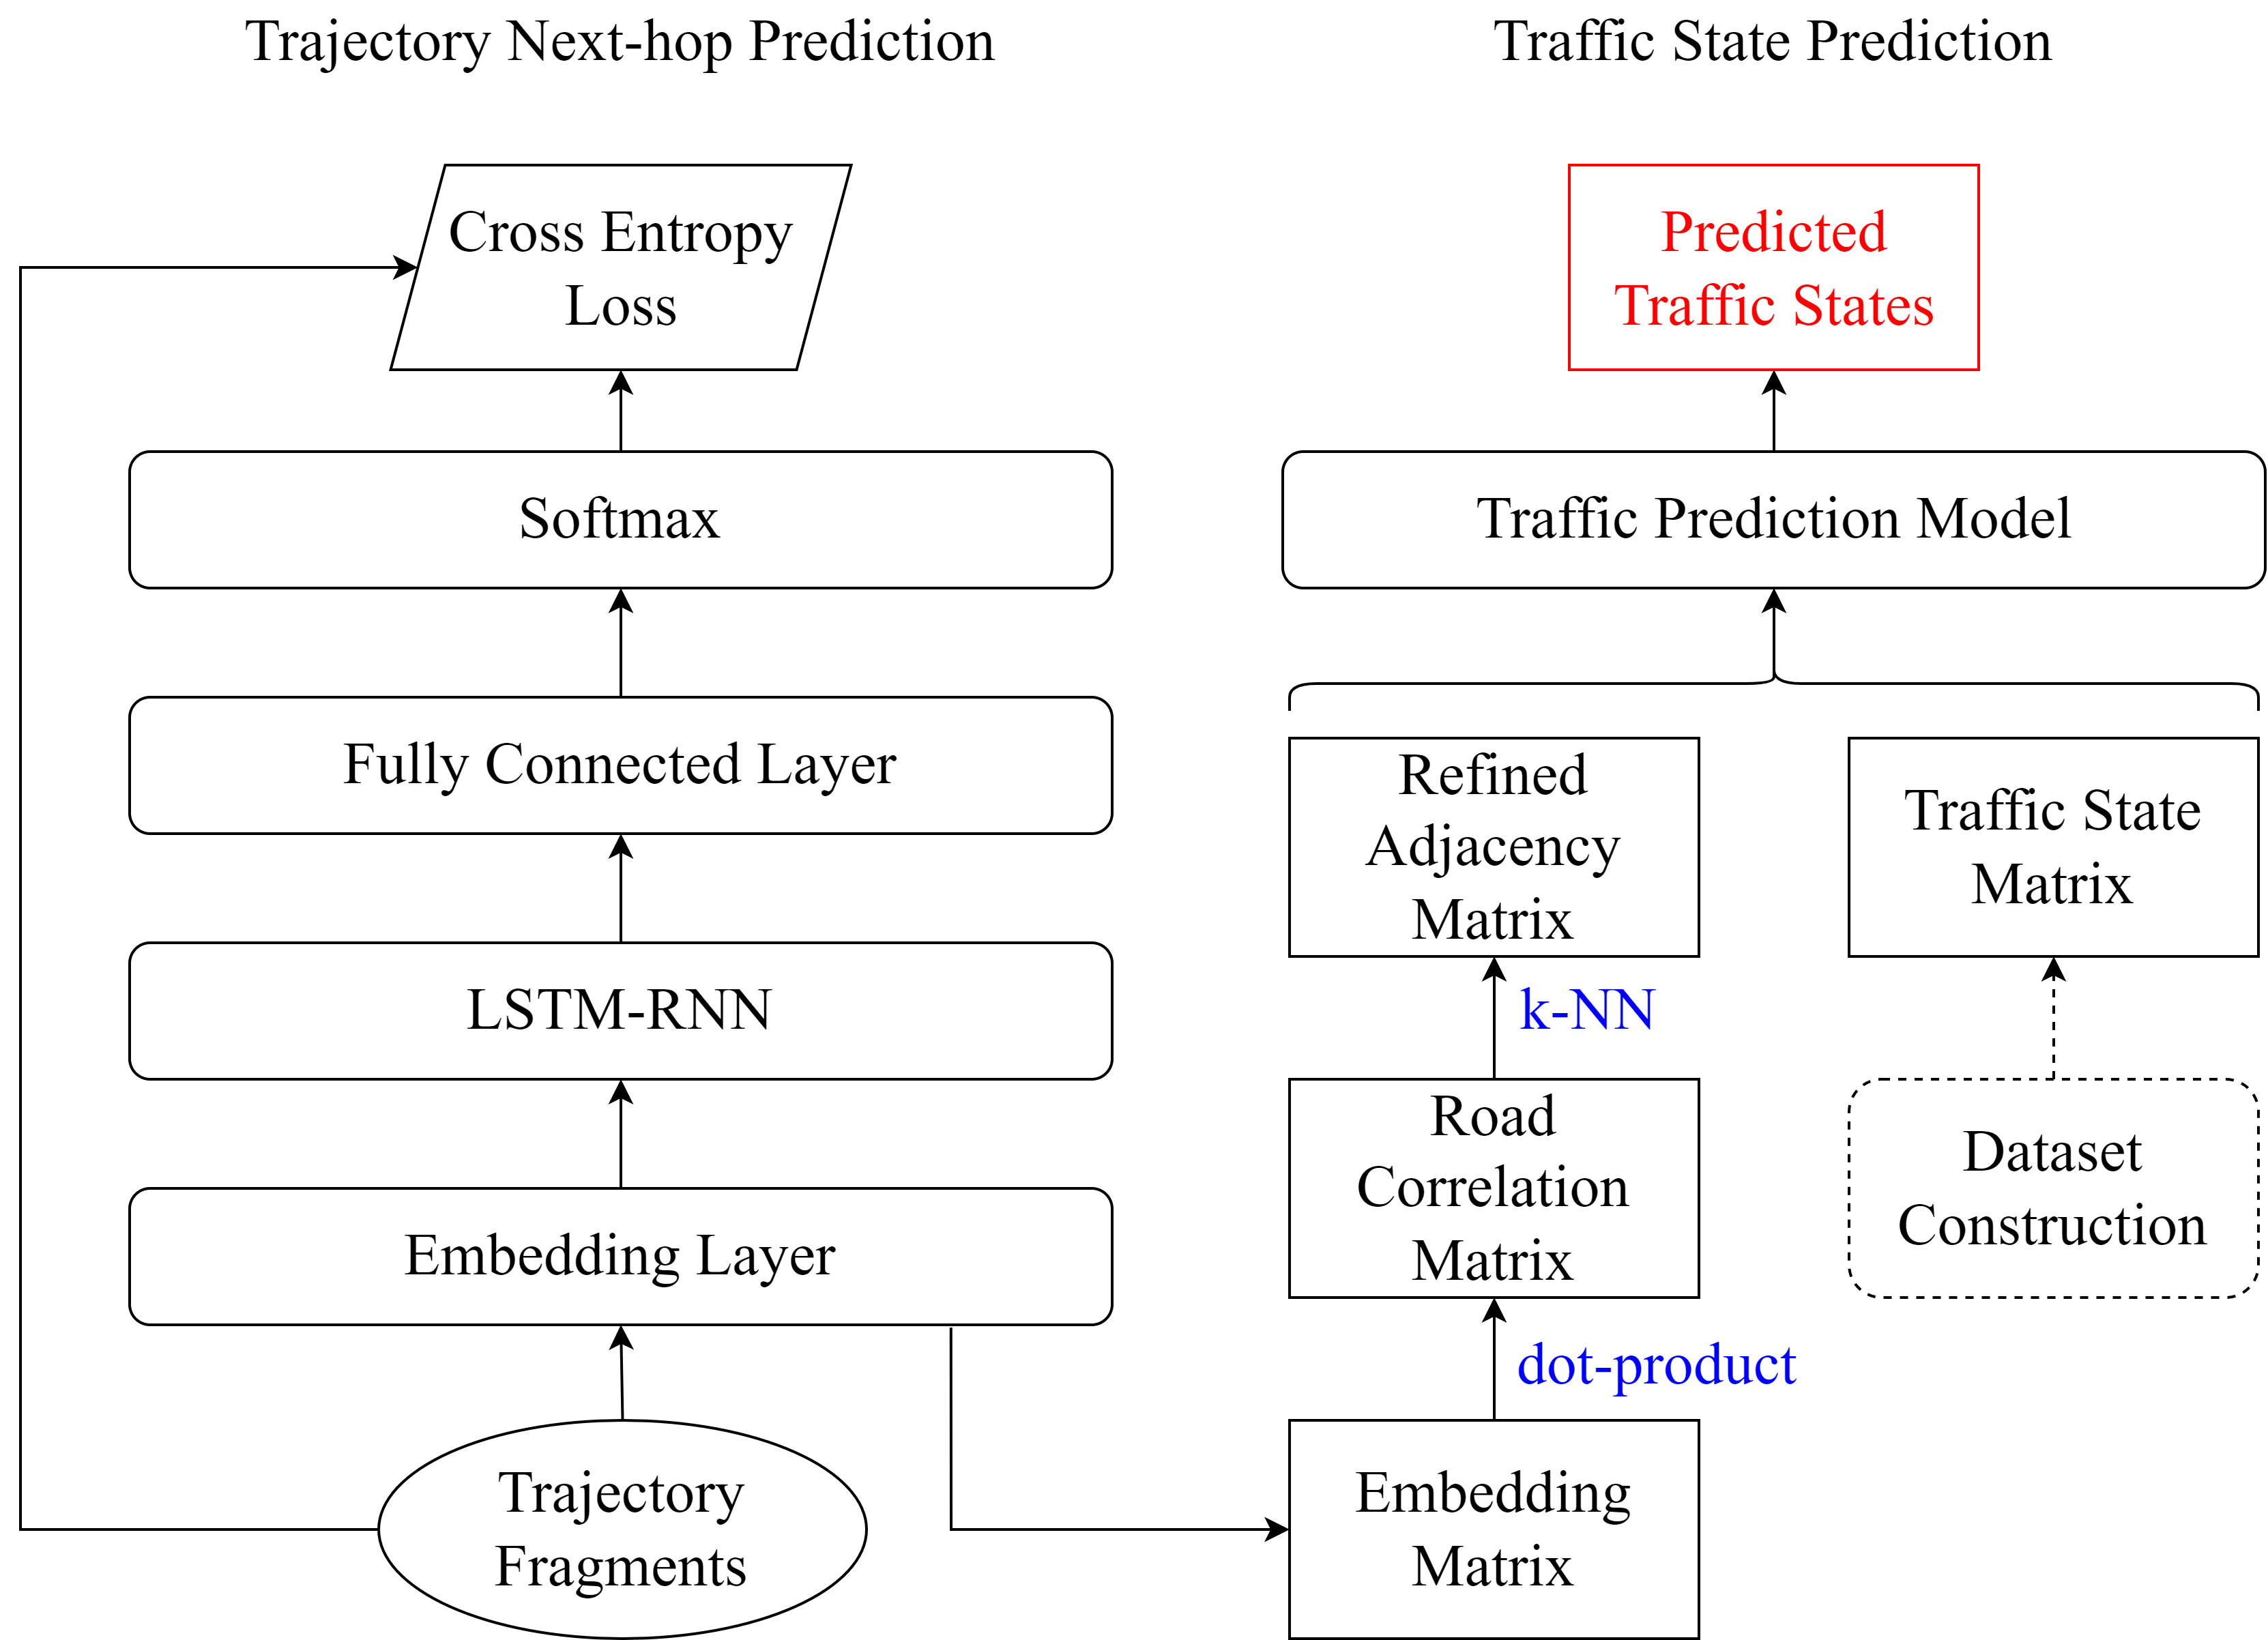
\includegraphics[width=\textwidth]{images/model.drawio.png}
    \caption{An overview of model structure.}
    \label{fig: model}
  \end{figure}

\subsection{Trajectory-based Road Correlation}
As mentioned in section 1, traffic states in real world varies over time. The traffic states in peak hours will even be completely different from other time intervals. However, most GCN models view the road network as a changeless graph, thus, they use adjacency matrix $A$ to represent it. On the contrary, trajectories indicate the route of vehicles, i.e. the real choices made by driver, which will give us the concrete transfer processes among roads. By leveraging them, we target to extract the road correspondence information inside transition and use a number to represent it. A simple way is regarding it as a first-order Markov process\cite{AAAI21}, and calculate the Markov transition probability as road correlation value by iterating on all trajectories. But Markov process is short in modeling high-order transition, since the next step is only related to the previous one, by its definition. Therefore, instead of statistical methods that result in a fixed probability value, we take advantage of deep leaning to let the machine automatically learn the transition process and output the high-order dependencies. To be specific, our idea is to build a trajectory next-hop prediction model and dynamically learn a vector representation of each road. Then compute vector similarity as road correlation. Details of methods and their rationale are introduced in the following paragraphs.

\vspace{\baselineskip}

\textbf{Migrating Word Embedding to Road Network Graph.} In NLP area, how to obtain the effective representations of text words has long been a research focus. One-hot embedding is a simple solution to represent each word with a one-hot vector whose dimension is equal to the size of vocabulary. The difference between these vectors are the word indexes. However, one-hot embedding suffers from dimension curse, making the embedding vectors very large and sparse. More importantly, the vectors cannot reflect the semantic relationships between words. Therefore, word embedding technologies\cite{word_embed} are proposed to efficiently learn a fixed-length real-value vector representation for each word. And the biggest advantage is that it can catch the contextual similarity of words. If two embedding vectors are close, i.e. have a high similarity, then the two corresponding words also tend to have similar semantic meanings.

In our work, a trajectory contains a sequence of different road IDs, which is similar to a sentence. Therefore, it is natural to treat each road as a word and use an embedding vector to represent it. What's more, we are inspired that road correlation can be modeled by the contextual similarity of words. To be specific, the similarity of words' semantic meanings ideally models the low and high-order dependency among roads, which perfectly meets the definition of road correlation. As a result, for road $r_1$, $r_2$ and their word embedding vectors $\mathbf{e_1}$ and $\mathbf{e_2}$, we define the road correlation function $Cor$ as the dot-product similarity\cite{dot_prod_simi} of the embedding vectors.
\begin{equation}
    Cor(r_1, r_2)=\mathbf{e_1}\cdot \mathbf{e_2}
\end{equation}

\vspace{\baselineskip}

\textbf{Next-hop Prediction Model}. To learn the embedding vectors, we propose a simple LSTM\cite{LSTM}-based model to predict the next-hop of a trajectory. Firstly, to utilize the trajectories, we use a sliding window strategy to generate training samples. After extracting the road sequence as $T^r=\{r_1, r_2, \dots, r_l \}$, we can obtain $l-w$ fragments by sliding a window with size $w$. A fragment is denoted as $\{r_1, r_2, \dots, r_w\}$, as well as its corresponding next-hop $r_{w+1}$. Next, we feed the fragments into an embedding layer that uses an embedding matrix $E\in\RR^{n_r\times d_r}$ to map each road ID to a vector of continuous values, where $n_r$ is the number of roads and $d_r$ is the embedding dimension. The second layer is an LSTM-RNN to capture dependencies in the sequence. LSTM encodes the embedded fragment into a single hidden vector with dimension $d_h$ after $w$ steps' iteration. The last layer is a fully connected linear layer that converts the hidden vector to an output length-$n_r$ vector for classification. Then use \textit{Softmax} function to generate the probability distribution. Cross entropy is served as loss function. The procedure of forward propagation is given in the following equations.
\begin{equation}
    \begin{aligned}
        \mathbf{e}&=\mathrm{Embedding}(r)\\
        h&=\mathrm{LSTM}(\mathbf{e})\\
        o&=W^\mathsf{T}h+b\\
        \hat P&=Softmax(o)\\
        \mathcal{L}&=CrossEntropy(\hat P, P)
    \end{aligned}
\end{equation}

After training, we take out the embedding matrix $E$ in the embedding layer and calculate the \textbf{road correlation matrix} as
\begin{equation}
    C=E\cdot E^\mathsf{T}
\end{equation}
where $C_{i, j}=\mathbf{e_i}\cdot \mathbf{e_j}=Cor(r_i, r_j)$.

\subsection{Improving Traffic State Prediction}
Most state-of-the-art GCN models for traffic prediction take two inputs. One is traffic states, which is $X$ in our work. The other is graph adjacency matrix $A$ where information is shared and propagated along the edges. As stated in section 1, the advantage of correlation matrix is that it can reflect the dependencies among roads in real world, which is an improved version of adjacency. Therefore, instead of making a brand-new model, we decide to integrate road correlation matrix $C$ into the existing models to give them the correlation knowledge that will benefit in prediction. A naive thought is to replace adjacency matrix by road correlation matrix since they have the same shape $n_r\times n_r$. However, practice proves that this does not work well, and binary relations are still necessary. Therefore, we proposed a procedure to refine the adjacency matrix via the idea of $k$-nearest neighbors ($k$-NN)\cite{knn}. In detail, the semantic distance among roads can be represented by the distance of their embedding vectors, which is negatively related to the similarity, i.e. $distance(r_1, r_2)=-Cor(r_1, r_2)$. Therefore, finding the $k$ nearest neighbors of a road $r_i$ is equal to find the $k$ biggest correlation values' indices in the $i$-th row of road correlation matrix $C$. The \textit{refined adjacency matrix} $A'\in[0, 1]^{n_r\times n_r}$ will be determined as
\begin{equation}
    A'_{i, j}=\mathbb{I}(r_j\in k\mathrm{-NN}(r_i))=\mathbb{I}(j\in \mathrm{argsort}(C_i)_{:k})
\end{equation}
where $\mathbb{I}$ stands for the indicator function, $k\mathrm{-NN}$ generate a set of $k$ nearest neighbor roads, and $C_i$ is the $i$-th row of the correlation matrix. The order of $\mathrm{argsort}$ function is descending.

By replacing $A$ with $A'$, we improve the accuracy of traffic prediction models. The details of empirical verification is given in the next section.
